%!TEX root = ../../thesis.tex
\section{WebSockets}
\label{realtime-ws}

Websockets (WS) is a technology that adds a full-duplex\footnote{Full-duplex means that both sites are able send messages simultaneously.} communication channel between browser and server. WS stands for two things: 1) the WebSocket protocol itself and 2) the WebSocket API, an interface in the browser. The WS protocol has been designed to work as a general communication protocol and is not limited to a client-server scenario.

\begin{figure}[htb]
  \centerline{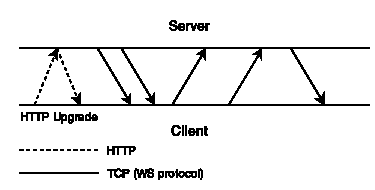
\includegraphics[width=0.9\linewidth]{images/Websockets.pdf}}
  \caption[Websocket communication]{Websocket communication}
  \label{fig:websockets}
\end{figure}

\reffigure{fig:websockets} shows the communication structure of a WS connection. All data is sent through an open TCP connection that is created after an initial handshake and negotiation through a HTTP Upgrade request from the client. This negotiation does not strictly rely on HTTP as handshake protocol but must be used by browsers as there is no browser API to create a TCP connection. In alternate setups (e.g. server to server WS), the negotiation can be based on any protocol, yet using HTTP has additional advantages. When HTTP is used for the handshake, it can be assured that WS works in any environment that is capable of using HTTP. Therefore both sides can use port 80 for the communication (respectively port 443 for secure connections) which are not blocked by most firewalls \cite[p. 298f]{grigorik2013high}. This enables developers to use WS in a variety of already existing environments without the need of altering firewall settings. The socket negotiation includes the exchange of environment keys, lists of supported protocol extensions and subprotocols as well as the protocol version. Once the handshake is complete, both sites can send and receive messages through the TCP connection. Messages do not require a request/answer pattern as with HTTP and can be sent asynchronously. This makes applications flexible and fast but also requires developers to adapt to a fully asynchronous message protocol \cite[chapter: Use Cases]{ubl2010websockets}.

\begin{lstlisting}[language=JavaScript, caption=Connecting to and using Websockets, label=lst:websockets]
  var ws = new WebSocket("ws://myserver.com/websocket");
  
  ws.onopen = function(){
    // connection established
    ws.send("hello server");
  };

  ws.onmessage = function(event) {
    console.log("new message", event.data);
    ws.close(); // ends the connection
  };

  ws.onerror = function(event){
    console.log("something went wrong", event);
  };
\end{lstlisting}

The browser's WS API is simple to use because it hides most of the protocol's complexities from the developer. Creating a WS connection to a server does not require a manual HTTP Upgrade request. It is entirely handled by the \code{WebSocket} object and its constructor as shown in \reflisting{lst:websockets} (line 1). All events trigger the attached event handlers in the same way that, say, DOM events trigger their events, so developers can use the same patterns here. The \code{onopen} trigger (line 3ff) informs the client that the connection has been established and it is now possible to send and receive messages. A client can send messages with the WS object's \code{send} method. The plain WS protocol does not support named message events like the SSE (see \refchapter{realtime-sse}) but they can be added manually by including the name of the event into the message itself. Once again, the WS object abstracts greatly from the WS protocol because messages are internally sent as so-called ``frames'' instead of simple strings. Frames are binary messages that encapsulate the data and contain the meta information of the messages (e.g. the length)\cite[p. 43ff]{wang2013websockets}. However, there is no way to reach to the frame level through the browser WS API.

The \code{onmessage} handler (line 8ff) is triggered when a server message arrives at the client. The \code{event} object, which is passed to the handler as the first parameter, contains the message content in its \code{data} property. If an error occurs somewhere in the communication, the \code{onerror} (line 13ff) handler is executed and more details about the error are handed in via the event object, so developers can react to any problem appropriately.

One advantage of WS over SSE, aside from supporting full-duplex communication, is its capability to send binary data. This means that client and server could use a fully custom protocol that is optimized for the specific use case of the application. In general, client and server have to agree on a custom protocol because there are no standardized messages or idioms like REST for the communication. However, WS was not introduced to replace XHR, which remains the first choice for web developers when it comes to data exchange with a server. WS was built for modern web applications with the need for push notifications or real-time communication in addition to normal HTTP requests.